%Fiquemos com Deus e Nossa Senhora!
%Sao Jose de Cupertino rogai por nos!!
% ### Uses XeLaTeX ### %
% ### Needs beamer-master ### %
\documentclass[aspectratio=169]{beamer} %. Aspect Ratio 16:9

\usetheme{AI2} % beamerthemeSprace.sty
\usepackage[portuguese]{babel}
\usepackage[utf8]{inputenc}
\usepackage[T1]{fontenc}
\usepackage{ragged2e,gensymb}

\DeclareMathOperator*{\argmin}{arg\,min}
\DeclareMathOperator*{\argmax}{arg\,max}
\DeclareMathOperator{\sign}{sgn}

% DATA FOR FOOTER
\date{2021}
\title{- $k$-Vizinhos mais Próximos}
\author{João Paulo Papa}
\institute{Advanced Institute for Artificial Intelligence (AI2)}

\begin{document}
% ####################################
% FIRST SLIDE 						:: \SliTit{This is the Title of the Talk}{A. B. Name}{Sprace}
% SUB-TITLE SLIDE 					:: \SliSubTit{<title>}{<explanation}
% SUB-SUB-TITLE SLIDE				:: \SliSubSubTit{<title>}{<explanation}
% SLIDE WITH TITLE 					:: \SliT{Title}{Content}
% SLIDE NO TITLE 						:: \Sli{Content} 
% SLIDE DOUBLE COLUMN WITH TITLE 	:: \SliDT{Title}{First Column}{Second Column}
% SLIDE DOUBLE COLUMN NO TITLE 		:: \SliD{First Column}{Second Column}
% SLIDE ADVANCED WITH TITLE 			:: \SliAdvT{Title}{Content}
% SLIDE ADVANCED NO TITLE 			:: \SliAdv{Content}
% SLIDE ADVANCED DOUBLE WITH TITLE 	:: \SliAdvDT{Title}{First Column}{Second Column}
% SLIDE ADVANCED DOUBLE NO TITLE 	:: \SliAdvD{First Column}{Second Column}
% SLIDE BLACK						:: \Black{ <Content> }
% SLIDE WHITE						:: \White{ <Content> }
% ITEMIZATION 						:: \begin{itemize}  \iOn{First} \iTw {Second} \iTh{Third} \end{itemize}
% COMMENT TEXT				 		:: \note{<comment>}
% SECTION 							:: \secx{Section} | \secxx{Sub-Section}
% BOLD SPRACE COLOR				:: \bfs{<text>}
% TABLE OF CONTENT					:: \tocitem{<title>}{<content>}
% LEFT ALIGN EQUATION				:: \begin{flalign*}  & <equation> &   \end{flalign*}
% CENTER ALIGN EQUATION	S			:: \begin{gather*} <equations>  \end{gather*}
% SLASH								:: \slashed{<>}
% BAR								:: \barr{<letter>} instead of \bar{<letter>}
% THEREFORE						:: use \portanto (larger and bold}
% 2 or 3 MATH SYMBOLS				:: \overset{<up>}{<down>} &  \underset{<below>}{\overset{<above>}{<middle>}}  
% INSERT TEXT IN FORMULA			:: \ins{<text>}
% EXERCISE							:: \exe{<exercise #>}{<exercise text>}
% SUGGESTED READING BOX			:: \sug{<references>}
% CITATION							:: \cittex{<citation>}
% CITATION DOUBLE COLUMN 			:: \cittexD{<citation>}
% TEXT POSITION						:: \texpos{<Xcm>}{<Ycm>}{<text>} origin = center of slide : x right | y down
% REFERENCE AT BOTTOM  S/D SLIDE		:: \refbotS{<reference>} \refbotD{<reference>}
% HIDDEN SLIDE						:: \hid
% COLOR BOX 						:: \blu{blue} + \red{rec} + \yel{yellow} + \gre{green} + \bege{beige}
% FRAME 							:: \fra{sprace} \frab{blue} \frar{red} + \fray{yellow} + \frag{green}		
% FIGURE 							:: \img{X}{Y}{<scale>}{Figure.png} 
% FIGURE							:: \includegraphics[scale=<scale>]{Figures/.png}
% FIGURE DOUBLE SLIDE NO TITLE		::  \img{-4}{0.5}{<scale>}{Figure.png} % Image 1st half
%									::  \img{4}{0.5}{<scale>}{Figure.png} % Image 2nd half
% FIGURE DOUBLE SLIDE WITH TITLE		::  \img{-4}{0}{<scale>}{Figure.png} % Image 1st half
%									::  \img{4}{0}{<scale>}{Figure.png} % Image 2nd half
% INCLUDING SWF (Flash)				:: \usepackage{media9} and \includemedia >> USE ACROBAT <<
%%%%%%%%%%%%%%%%%%%%%%%%%%%%%%%%%%%%%%%%%%%%%%%%%%
% ###############################################################################
% FIRST SLIDE
\SliTit{{\LARGE $k$-Vizinhos mais Próximos}}{Advanced Institute for Artificial Intelligence -- AI2}{https://advancedinstitute.ai}
%%%%%%%%%%%%%%%%%%%%%%%%%%%%%%%%%%%%%%%%%%%%%%%%%%
% ###############################################################################
% SLIDE SUB-TITLE
%\SliSubTit{Sub-Title}{Description}{}
%%%%%%%%%%%%%%%%%%%%%%%%%%%%%%%%%%%%%%%%%%%%%%%%%%
% ###############################################################################
%\SliSubSubTit{Sub-Sub-Title}{Description}
 %%%%%%%%%%%%%%%%%%%%%%%%%%%%%%%%%%%%%%%%%%%%%%%%%%


\SliT{Introdução}{

\justifying Uma das técnicas mais tradicionais em aprendizado de máquina é conhecida por $k$-Vizinhos mais Próximos, do inglês \emph{k-Nearest Neighbours} - $k$-NN. Esta técnica é uma generalização de outra mais antiga conhecida por Vizinhos mais Próximos, do inglês \emph{Nearest Neighbours} - NN. Ambas são abordagens bastante simples, pois \textbf{não existe etapa de treinamento}, muito embora tenhamos ainda o conjunto de treinamento. 
}

\Sli{
\justify \underline{Definição do problema:} dado um conjunto de treinamento rotulado com $m$ amostras ${\cal X}^1 = \{(\boldsymbol{x}_1,y_1),(\boldsymbol{x}_2,y_2),\ldots,(\boldsymbol{x}_m,y_m)\}$, queremos classificar corretamente uma amostra $\boldsymbol{x}\in{\cal X}^2$.

\justify \underline{Objetivo:} dada uma amostra $\boldsymbol{x}$ qualquer do conjunto de teste, o seu rótulo $y$ será o mesmo da amostra mais próxima do conjunto de treinamento, ou seja, aquela que satisfaz a seguinte equação:

\begin{equation}
	y = \argmin_{y_i|\boldsymbol{x}_i\in{\cal X}^1}\norm{\boldsymbol{x}-\boldsymbol{x}_i}_2.
\end{equation}
}

\Sli{
\justify Vejamos um exemplo do funcionamento da técnica NN.

\begin{center}
\begin{tabular}{ccc}
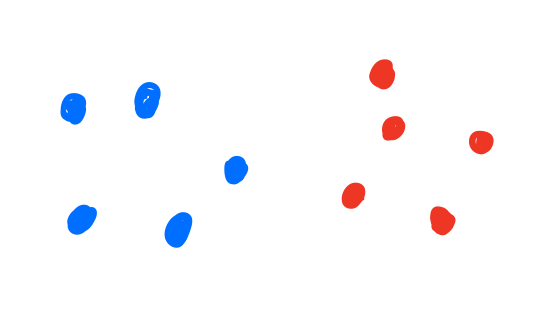
\includegraphics[scale=0.23]{./figs/KNN_Fig1.png} &
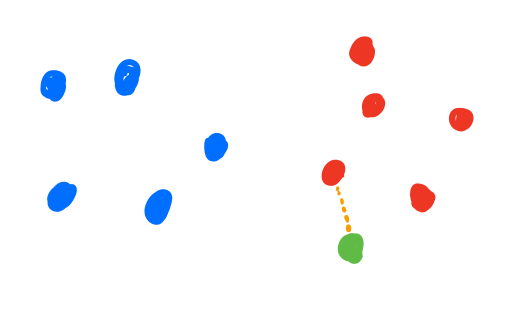
\includegraphics[scale=0.23]{./figs/KNN_Fig2.png} &
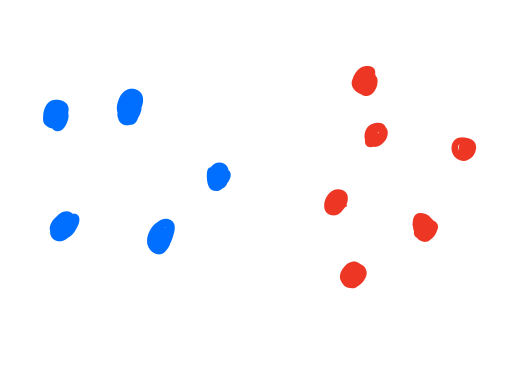
\includegraphics[scale=0.23]{./figs/KNN_Fig3.png} \\	
Conjunto de treinamento & Amostra a ser classificada & Amostra classificada
\end{tabular}
\end{center}
}

\Sli{
\justify Quando o conjunto de dados está "bem comportado", NN é uma das melhores técnicas a serem utilizadas. No entanto, isso nem sempre acontece. Problema? "Ruídos" no conjunto de dados de treinamento.

\begin{center}
\begin{tabular}{ccc}
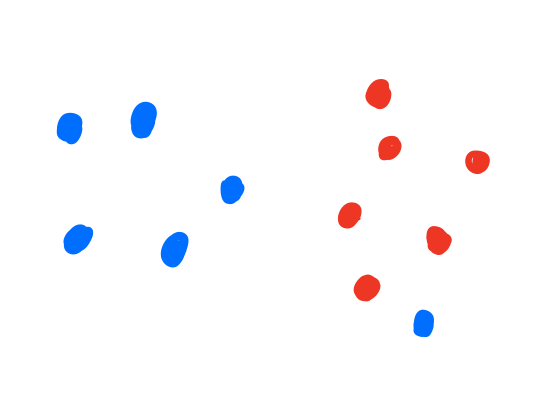
\includegraphics[scale=0.23]{./figs/KNN_Fig4.png} &
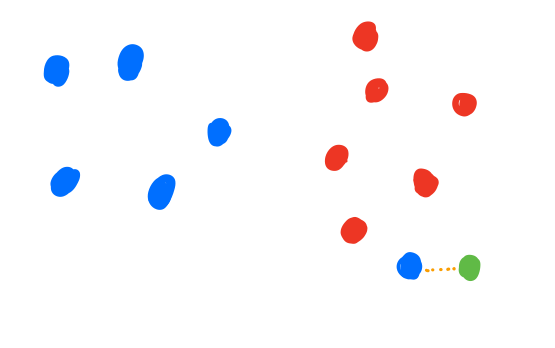
\includegraphics[scale=0.23]{./figs/KNN_Fig5.png} &
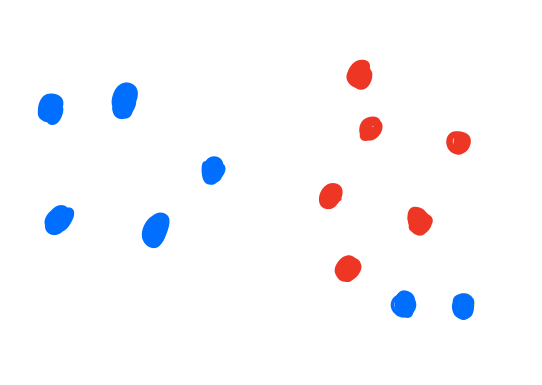
\includegraphics[scale=0.23]{./figs/KNN_Fig6.png} \\	
Conjunto de treinamento & Amostra a ser classificada & Amostra classificada
\end{tabular}
\end{center}
}

\Sli{
Uma generalização da técnica NN seria, então, conectar a amostra de teste aos seus $k$ vizinhos mais próximos, dando origem ao classificador $k$-NN. Desta forma, considerando o exemplo anterior, a amostra seria corretamente classificada caso considerássemos $k=3$, por exemplo (geralmente utilizamos valores ímpares para $k$ para evitarmos desempates).

\begin{center}
\begin{tabular}{ccc}
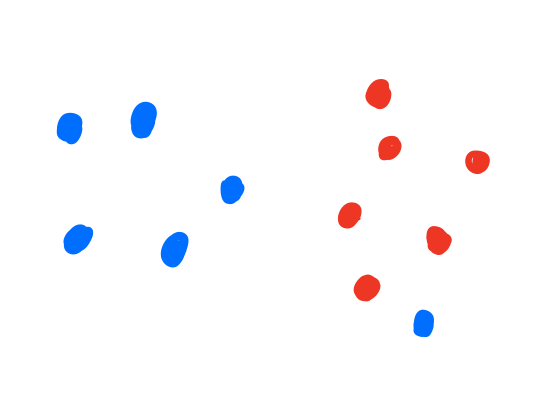
\includegraphics[scale=0.23]{./figs/KNN_Fig4.png} &
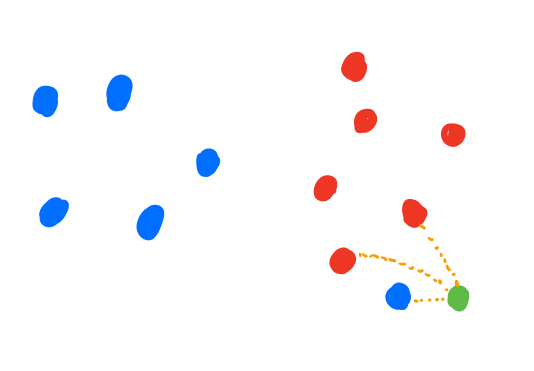
\includegraphics[scale=0.23]{./figs/KNN_Fig7.png} &
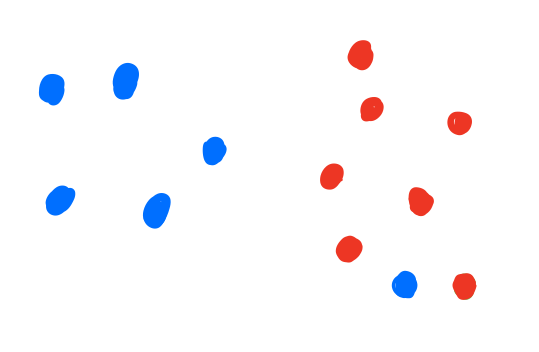
\includegraphics[scale=0.23]{./figs/KNN_Fig8.png} \\	
Conjunto de treinamento & Amostra a ser classificada & Amostra classificada
\end{tabular}
\end{center}
}

\Sli{
\justify A técnica $k$-NN é interessante para problemas de \textbf{recomendação} e \textbf{recuperação}, dado que faz uso das amostras mais próximas para tomada de decisão. Esses dados podem ser, então, utilizados para fins de recomendação. Outro ponto importante diz respeito à \textbf{regressão} por $k$-NN, que também é bastante simples. Neste caso, ao conectar à amostra de teste aos seus $k$ vizinhos mais próximos, basta utilizar, por exemplo, o valor médio de suas saídas como sendo o valor a ser estimado.
}

\SliT{Variantes}{
\justify Uma variante conhecida da técnica $k$-NN é a sua versão \textbf{ponderada}, conhecida por \emph{weighted $k$-NN}. A ideia consiste em associar pesos à cada um dos $k$ vizinhos mais próximos, que podem ser, por exemplo, o \textbf{inverso de sua distância} para a amostra em questão. Esses pesos são normalizados e utilizados para ponderar a decisão. A ideia é que amostras mais longes tenham menos influência durante o processo de decisão.
}

\Sli{
Vejamos um exemplo do $k$-nn ponderado versus a sua versão tradicional.

\begin{center}
\begin{tabular}{ccc}
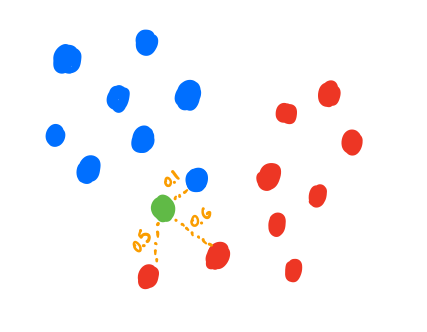
\includegraphics[scale=0.23]{./figs/KNN_Fig9.png} &
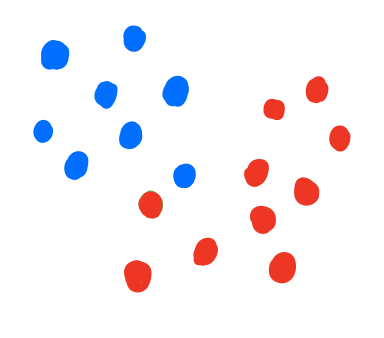
\includegraphics[scale=0.23]{./figs/KNN_Fig10.png} &
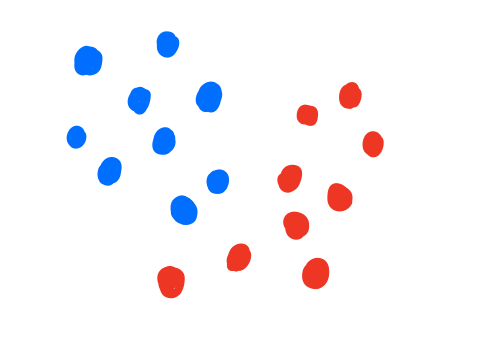
\includegraphics[scale=0.23]{./figs/KNN_Fig11.png} \\	
Conjunto de treinamento & Classificação por $k$-NN & Classificação por $k$-NN ponderado \\
\end{tabular}
\end{center}
Seja $\boldsymbol{w}\in\mathbb{R}^3$ o vetor de pesos, tal que $w_1 = 1/0.1$ (classe azul), $w_2 = 1/0.5$ (classe vermelha) e $w_3 = 1/0.6$ (classe vermelha). Normalizando os mesmos, temos que $w_1 = 0.74$, $w_2=0.17$ e $w_3 = 0.09$. Muito embora a amostra verde esteja ligada às duas amostras da classe vermelha, o peso desta classe ($w_2+w_3 = 0.26$) é menor do que aquele dado pela amostra da classe azul, ou seja, $w_1 = 0.74$. 
}

\end{document}